\documentclass[12pt,twoside,a4paper]{report}
\usepackage{amsmath}
\usepackage{amssymb}
\usepackage[style=ieee]{biblatex}
\addbibresource{references.bib}
\usepackage{graphicx}
%% Times new roman font
%\usepackage{mathptmx}
%% Arial font
%\usepackage{helvet}
%\renewcommand{\familydefault}{\sfdefault}
\usepackage{hyperref}
\usepackage[all]{hypcap}
\title{Detecting abnormalities on chest X-rays using deep neural networks}
\author{
  Swaroop Kumar M L\\
  Department of Studies in Computer Science\\
  University of Mysore
}
\date{\today}
\begin{document}
\maketitle
\begin{abstract}
  Diseases like pneumonia and tuberculosis are leading causes of death
  world-wide. Although conclusive diagnosis requires other tests such as a
  sputum culture, chest radiography can be an important diagnostic aid and is
  routinely recommended since it is fast, affordable and highly sensitive.
  Moreover, automated detection of abnormalities on the chest X-ray can help in
  active case finding, screening, and in cases where other tests are not
  available or are inconclusive. Due to the nature of the domain, it is also
  important that algorithms not only make inferences
  but also generate explanations sufficient to convice a human expert.\\

  Inspired by previous work, we develop algorithms that can detect abnormalities
  on the x-ray. The algorithm explains these detections by generating heatmaps
  pointing out areas of the image that most influenced it. We establish
  baselines, benchmark against previous work and show that a) transfer-learning
  from a large non-TB dataset dramatically improves TB detection, b) models in
  the domain show inferior performance on external data from a different
  hospital system but c) recent techniques such as mixup and progressive
  resizing improve performance and generalization. We achieve performance
  competitive with previous work in detecting pneumonia-like and other
  abnormalities on the NIH chestX-ray14 dataset and in detecting tuberculosis on
  the Shenzhen hospital dataset, and achieve state-of-the-art performance on the
  Montgomery county tuberculosis dataset. We evaluate our algorithms on
  bacterial and viral pneumonia separately, look for potential sources of bias
  and test our baseline with respect to gender, age and view position.
\end{abstract}
\tableofcontents
\chapter{Introduction}
\section{Problem definition}
The lungs are made up of small air-sacks called alveoli. When, for example, air
in the alveoli is replaced with pus, blood and other fluids, referred to as
consolidation and commonly caused by pneumonia, or when abscesses in the lung
rupture forming cavities, indicating a tuberculosis infection, these are
visible on the chest x-ray. See figure \ref{basic_examples} for examples.\\

Radiologists are trained to look for signs of these abnormalities, use subtle
visual features to differentiate among the various types, reason about their
causes and help in diagnosis and treatment. An algorithm that can automatically
detect these abnormalities can be useful in numerous ways (see section
\ref{motivation}).\\
% \begin{enumerate}
% \item{Helping to actively find patients who may be infected with a particular
%   disease in the general population }
% \item{As an initial screening test before other, less affordable tests}
% \item{Prioritizing patients for subsequent review by a trained radiologist or
%   aiding a radiologist in other ways by being part of her workflow }
% \end{enumerate}
\begin{figure}
  % \fbox{
  % \begin{minipage}{\textwidth}
  \centering
  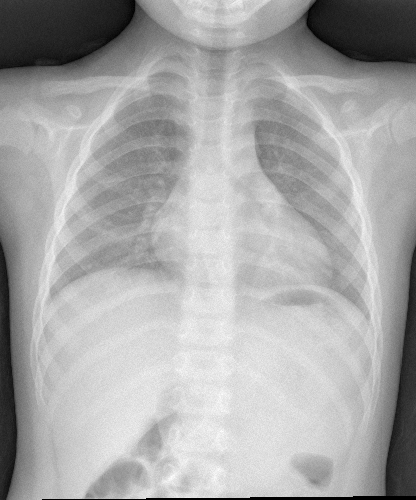
\includegraphics[width=0.3\textwidth]{images/normal1}\hspace{0.01\textwidth}%
  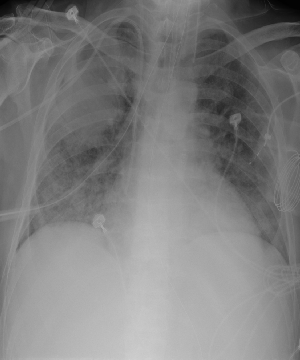
\includegraphics[width=0.3\textwidth]{images/consolidation_original}\hspace{0.01\textwidth}%
  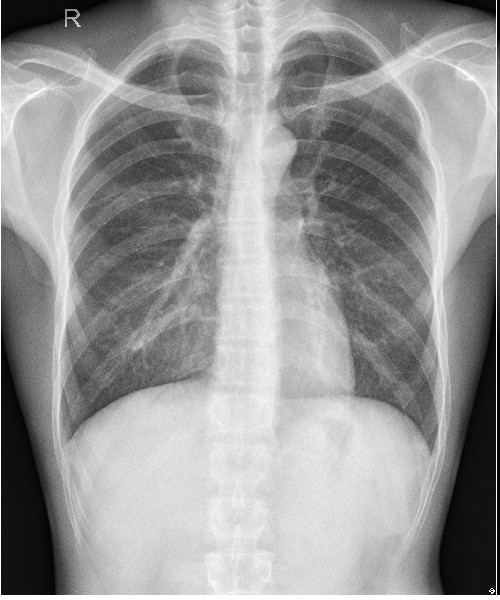
\includegraphics[width=0.3\textwidth]{images/TB_original}\\[0.01\textwidth]
  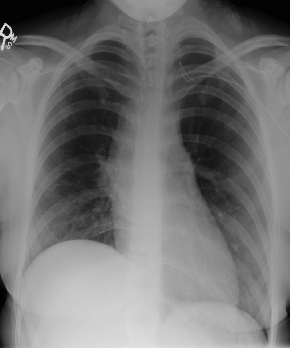
\includegraphics[width=0.3\textwidth]{images/normal2}\hspace{0.01\textwidth}%
  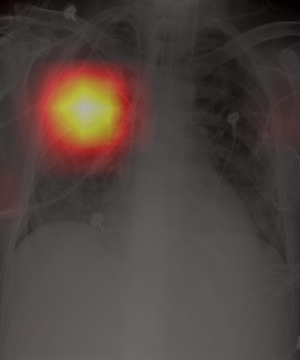
\includegraphics[width=0.3\textwidth]{images/consolidation_heatmap}\hspace{0.01\textwidth}%
  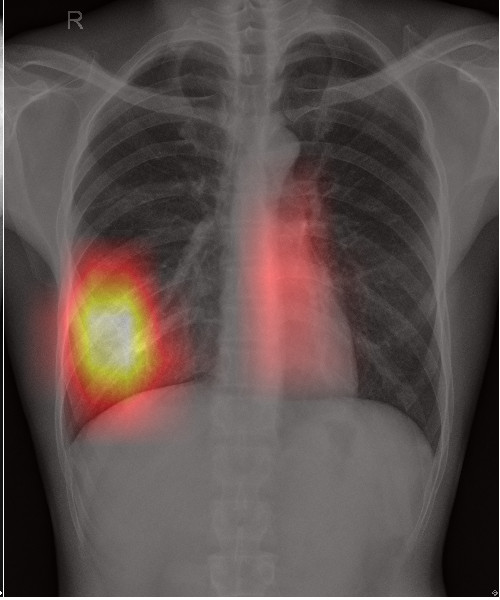
\includegraphics[width=0.3\textwidth]{images/TB_heatmap}
  \caption{From left to right: The first column shows two \emph{Normal} images.
    Columns 2 and 3 show images with \emph{Pneumonia} and \emph{Tuberculosis}
    respectively, the first row showing the original images and the second
    showing the same overlaid with heatmaps localizing the abnormalities, which
    we call \emph{explanations}}
  % \end{minipage}
  % }
  \label{basic_examples}
\end{figure}

However, building the hardware and software infrastructure for a clinically
relevant system that is useful in practice is a problem which presents unique
challenges of its own\footnote{We discuss possible implementations in section
  \ref{practical}}. Our work focuses on the core algorithm. We divide the
problem into, and explore, four sub-problems.
\pagebreak[4]
\subsection{Classification}
    
For our primary dataset, a large collection of chest x-rays annotated with
multiple abnormalities including pneumonia \cite{Wang2017a} (see section
\ref{nih_cxr}), we formulate the problem as a multi-class multi-label
classification problem. Given the $n$-dimensional input feature space $X =
\mathbb{R} ^n$, and a set of $c$ class labels corresponding to $c$ abnormalities
$L = \{\,l_1 ,l_2 ,l_3 \dots l_c\,\}$ the task is to learn a function $f:X
\rightarrow 2^L$ from the training set $D = \{\,(x_i, Y_i) \mid 1 \leq i \leq m
\,\}$. For each example $(x_i, Y_i) \in D$, $x_i \in X$ is an $n$-dimensional
feature vector $\{\, x_{i1}, x_{i2}, x_{i3} \dots x_{in} \,\}$, each feature
representing the intensity value of a single pixel of the input image, and $Y_i
\subseteq L $ is the set of abnormalities associated with $x_i$. For an unseen
instance $x$, the classifier $f(\cdot)$ predicts $f(x) \subseteq L$ as the set
of abnormalities for
$x$.\\

For the Shenzhen hospital tuberculosis dataset (see section \ref{szhenzhen}), we
formulate the problem as a binary classification problem. Again, suppose $X$ is
the $n$-dimensional input feature space. The task is to learn a function $f:X
\rightarrow \{\,0, 1 \,\}$ from the training set $D = \{\,(\,x_i, y_i) \mid 1
\leq i \leq m\,\}$. For each $(x_i, y_i) \in D$, $x_i \in X$ is an
$n$-dimensional feature vector $\{\,x_{i1}, x_{i2}, x_{i3} \dots x_{in}\,\}$,
each feature corresponding to the intensity value of a single pixel of the input
image, and $y_i \in \{\,0, 1\,\}$ is the corresponding label, $0$ meaning
\emph{normal} and $1$ meaning \emph{tuberculosis}. Given an unseen $x \in X$,
the classifier
$f(\cdot)$ predicts $f(x) \in \{\,0, 1\,\}$ as being the label for $x$.\\

In both cases, $f(\cdot)$ consists of a deep convolutional neural
network\cite{lecun1998gradient}, specifically a variant of
DenseNet\cite{iandola2014densenet} trained using the Adam\cite{kingma2014adam}
optimization algorithm (see sections \ref{architecture} and
\ref{training_procedure} for discussions about the model architecture and
training procedure). In the case of NIH ChestX-ray14, our primary dataset, the
output of the network is a 14-dimensional vector $P = \{\,p_1, p_2, p_3 \dots
p_{14}\,\}$ where $p_k \in P$ corresponds to the $k^{th}$ abnormality and $0
\leq p_k \leq 1$. A set of optimal thresholds $T = \{\,t_1, t_2, t_3 \dots
t_{14}\,\}$ is determined by maximizing the network's F1-score on the training
set and applied to the output of the network so that the final output $Y
\subseteq L$ is:
\begin{equation}
  Y = \{\,l_i \in L \mid p_i \in P \wedge t_i \in T \wedge p_i > t_i \,\}
\end{equation}
In the case of the Shenzhen hospital tuberculosis dataset, the output of the
network is a 2-dimensional vector $P = \{\,p_1, p_2\,\}$ where $0 \leq p_1 \leq
1$ and $0 \leq p_2 \leq 1$ and the final output $y$ is:
\begin{equation}
  y = 
  \begin{cases}
    0 & \text{if $p1 \geq p2$\, (normal)}\\
    1 & \text{if $p2 > p1$\, (tuberculosis)}
  \end{cases}
\end{equation}

\subsection{Explainability}
Deep neural networks have outperformed previous methods in several domains.
However, they remain black-boxes with millions of parameters, leading to a lack
of trust and limiting their use in routine clinical practice. Several methods
have been proposed to make these models more interpretable, broadly falling into
two categories:
\begin{enumerate}
\item{Methods that create a proxy model which behaves similarly to the original
    model, but is simpler and easier to understand. These include methods like
    LIME\cite{ribeiro2016should} and SHAP\cite{NIPS2017_7062}. While these
    methods are model-independent, they tend to be very slow.}
\item{Methods that generate a saliency map which highlights a small portion of
    the input which is most relevant, in a single forward and backward pass
    through the network. These include methods like LRP\cite{bach2015pixel},
    DeepLIFT\cite{shrikumar2017learning}, CAM\cite{zhou2016learning} and
    Grad-CAM\cite{selvaraju2017grad}.}
\end{enumerate}
We use the CAM method and use the term \emph{explanation} to mean a saliency map
or heatmap. Given an input $x = \{\, x_{1}, x_{2}, x_{3} \dots x_{n} \,\} \in
X$, and a set of class labels $L = \{\,l_1 ,l_2 ,l_3 \dots l_c\,\}$, the task is
to compute the attribution $A_j = \{\,a_{j1}, a_{j2}, a_{j3} \dots a_{jn}\,\}
\in \mathbb{R} ^n$ for each class $l_j \in L$ where $a_{ji} \in A$ is a measure
of the relevance of
the $i^{th}$ feature to the model's inference regarding the $j^{th}$ class.\\

The network consists of a fully convolutional DenseNet backbone followed by an
adaptive-average-pooling layer and a single fully-connected layer. The fully
convolutional part of the network results in $k$ $w$ x $h$ feature maps which
are averaged along the width and height to form a $k$ dimensional vector, which
is fed to the single fully-connected layer with $k$ input nodes and $c$ output
nodes. If $f_i$ is the $i^{th}$ feature map and $w^j _i$ is the weight between
the $i^{th}$ input node and the $j^{th}$ output node in the fully-connected
layer, the saliency map for the $j^{th}$ class $M_j$ is
\begin{equation}
  M_j = \sum _i \, w^j _i \, f_i
\end{equation}
$M_j$ is a $w$ x $h$ saliency map which is interpolated to the size of the input
image and measures the relevance of each pixel to the model's decision regarding
the $j^{th}$ class, and can be visualized as a heatmap (see figure
\ref{basic_examples}). This serves as an \emph{explanation} of the model's
inference, allowing physicians and radiologists to decide how much trust to
invest in it.

\subsection{Generalizability}
A test set is considered representative of data that will be encountered in the
external world and is used exclusively to evaluate a model. However, true
generalization to new datasets may be lower than expected.
\begin{enumerate}
\item{Since model design choices are based on previous work, methods in an
    application domain may overfit to one or a few popular datasets. However,
    \cite{recht2018cifar} shows that this is not the case for CIFAR-10 despite
    years of methods being tested on this dataset}
\item{Two datasets may have different distributions. In the context of
    biomedical imaging, datasets may be collected from different hospital
    systems and machines. For example, in \cite{zech2018variable}, Zech et al.
    show that models trained on data from one hospital system showed inferior
    performance on data from others.}
\item{The dataset used to train a model may have confounding variables that do
    not exist in other datasets. For example, in \cite{zech2018variable}, Zech
    et al. also show that CNNs were able to directly detect the hospital system
    and department within a hospital system from a chest radiograph where
    saliency maps showed high activation in image corners. Since different
    departments and machines within a hospital system have different prevalence
    of a disease, the model may leverage these spurious correlations and fail to
    generalize}
\end{enumerate}
Since we observed the same phenomenon as in \cite{zech2018variable}, of saliency
maps showing high activation in image corners, we evaluated our models on
external datasets from different hospital systems and studied how recent
techniques affected generalization.

\subsection{Fairness}
Machine learning systems are increasingly being deployed in settings where they
may inadvertently learn and leverage biases in the datasets, discriminate based
on race, gender, etc. and amplify existing social inequities. For example, in
\cite{bolukbasi2016man}, Bolukbasi et al. show that the popular word embedding
space Word2Vec encodes gender bias. In \cite{buolamwini2018gender}, Buolamwini
et al. show that facial recognition datasets are overwhelmingly composed of
light-skinned individuals and that commercial gender classification systems
performed worse for dark-skinned people and females, with a difference in
accuracy of more than 30\% between
light-skinned males and dark-skinned females.\\

There has been substantial work in the research literature on fairness in ML on
the development of statistical definitions of fairness
\cite{chouldechova2017fair,dwork2012fairness,hardt2016equality} and algorithmic
methods to measure and mitigate undesirable biases
\cite{agarwal2018reductions,hardt2016equality,kusner2017counterfactual}. A
simple measure against bias in various fields has been to hide variables like
gender and race from a model, but complex machine learning models learn to use
other correlated variables as proxy for hidden ones (for example, zipcode as
correlated with race and the word `women' in an institution's name as correlated
with the gender of its students\cite{dastin_2018}). Moreover, hiding sensitive
variables from researchers exacerbates the problem by limiting their ability to
quantify and mitigate these biases. For example, in
\cite{esteva2017dermatologist}, Estava et al. found that convolutional neural
networks are effective at detecting melanoma from images. However, without
labels for skin characteristics such as color, accuracy of the
model for different skin-types cannot be measured.\\

In this work, we measure the potential for discrimination by
\begin{enumerate}
\item{Measuring the correlation of various abnormalities with gender and age
    group}
\item{Training models with architectures similar to the abnormality detection
    model, to identify gender and age group from images alone.}
\end{enumerate}
We test our baseline model's performance across genders and age groups.
\section{Motivation\label{motivation}}
Pneumonia and tuberculosis are leading causes of death worldwide. According to
the world health organization, pneumonia disproportionately affects children,
accounting for 16\% of all deaths of children under the age of 5 years\cite{}.
Tuberculosis is more prevalent in countries where many people live in absolute
poverty\cite{} with limited access to healthcare and in 2017 alone, caused 1.6
million preventable deaths\cite{}.\\

The global End TB strategy aims for a 95\% reduction in deaths due to TB by 2035
compared with 2015. Similarly, the National Strategic Plan (NSP) 2017-2025 sets
out to achieve a rapid decline in deaths due to TB and emphasizes the importance
of active case finding, that is, detection of TB cases early by seeking out
people in targeted groups and scaling up cheap and high sensitivity TB
diagnostic tests. The NSP has recommended three tests: sputum smear microscopy,
chest x-ray and the new CB-NAAT\footnote{CB-NAAT or Cartridge Based Nucleic Acid
  Amplification Test is a molecular test and is
  known as GeneXpert outside India} test.\\

Conventionally, patients are screened for TB or pneumonia related symptoms,
sputum examinations are recommended for those with positive symptoms, and chest
x-rays are recommended for those who test negative in the sputum examination.\\

With automated detection, x-ray tests have the potential to be faster and
significantly more affordable. They can be massively scaled up and used
\begin{enumerate}
\item{For active case finding in high-risk populations, for example, with mobile
    x-ray vans\cite{modi_suresh_2019}}
\item{As an initial screening test before or along with other tests such as a
    sputum examination}
\item{To aid a radiologist in her workflow by sorting her queue based on
    severity, suggesting areas to consider in an image, providing a second
    opinion, etc.}
\end{enumerate}

Our motivation in this regard is to further the goal of making automated
abnormality detection systems such as ours clinically relevant by making them
more accurate and explainable, testing their ability to generalize to other
hospital systems and making sure they do not discriminate based on gender, age
group, etc.
\section{Previous work}

\section{Our work}
Short overview of our experiments and results. A condensed version of chapters
\ref{exp}, \ref{res} and \ref{bias}
\section{Report layout}
Overall layout of the rest of the report.
\chapter{Literature survey\label{litsurvey}}
\section{CheXNet and CheXNext}
\section{Weakly supervised learning}
The body of work around weakly supervised learning, and for our purposes, two
forms of it:
\begin{enumerate}
\item{Learning with inaccurate labels. For example, learning from labels which
    were generated algorithmically and which may therefore be inaccurate. Here,
    labels were extracted from radiology reports in natural language text.}
\item{Learning from imprecise labels. For example, learning to precisely
    localize objects or patterns with imprecise image-level labels. We use this
    to generate explanations.}
\end{enumerate}
\section{Explainability}
A short review of methods such as weakly supervised localization, LIME and SHAP
which have been developed for generating explanations.
\section{Fairness}
Methods to quantify learned bias along the lines of gender, race, etc.
\section{Learning at multiple scales}
Methods to effectively combine inferences from multiple scales.
\section{Attention}
Methods to allow models to selectively pay attention to parts of an image.
\section{Recurrent neural networls}
A number of papers have shown that using recurrent neural networks to
effectively make use of correlations between different abnormalities improves
performance.
\section{Generalizability}
Atleast one other paper has studied how models in this domain generalize to
other datasets. I describe their results.
\section{Other methods}
\section{Tuberculosis}
\chapter{Data}
Here I describe all the datasets we use, as well as how we split them, and where
and how we use k-fold cross validation
\section{NIH CXR-14\label{nih_cxr}}
The NIH chestX-ray 14 dataset, our primary dataset annotated with 14 different
abnormalities including pneumonia.
\subsection{Challenges and issues}
\section{Mendeley\label{mendeley}}
This is the Mendelay pneumonia dataset of CXRs of children under 5 years, which
we use to test generalization.
\section{Szhenzhen\label{szhenzhen}}
Szhenzhen and Montgomery county tuberculosis datasets. Shenzhen is used to train
models and Montgomery is used to test generalization.
\section{Montgomery\label{montgomery}}
\chapter{Baselines}
\section{Model architecture\label{architecture}}
\section{Training procedure\label{training_procedure}}
\section{Weakly supervised localization}
\subsection{Saliency map to bounding box}
\subsection{LIME as an alternative}
\chapter{Experiments\label{exp}}
\section{Data augmentation}
\section{Test-time augmentation}
\section{Higher resolution}
\section{Progressive resizing}
\section{Ensembling for scale-invariance}
\section{Ensembling saliency maps}
\section{Mixup}
\section{Self-training}
\section{Transfer learning for tuberculosis}
\section{Generalizability}
\chapter{Results\label{res}}
\section{Comparison metrics}
\section{Comparison to previous work}
\section{Comparison to human radiologists}
\subsection{Caveats with comparison to human radiologists}
\section{Other important factors}
Such as how well predicted probabilities correspond to actual severity,
localization, and time
\section{Examples}
\chapter{Bias\label{bias}}
\section{Gender}
\section{Age}
\section{View position}
\chapter{Conclusion}
\chapter{Future work}
\section{Limitations of proposed work}
\section{Avenues for further research}
\section{Practical implementation and clinical relevance\label{practical}}
\section{More recent datasets}
Such as CheXPert and PadChest \printbibliography
\end{document}
